\chapter{Tinjauan Pustaka dan Dasar Teori}
Bab ini akan membahas tinjauan pustaka yang mencakup penelitian-penelitian sebelumnya sebagai referensi untuk melaksanakan tugas akhir. Selain itu, akan dijelaskan tentang teori-teori yang menjadi dasar dalam pembuatan aplikasi tugas akhir.
\section{Tinjauan Pustaka}
% ================================= Penelitian Designing Gamification for Programming Learning Applications =================================
Gamifikasi telah terbukti menjadi strategi yang efektif dalam meningkatkan minat dan motivasi belajar. 
Berdasarkan beberapa studi yang ada, pengimplementasian gamifikasi yang tepat akan meningkatkan ketertarikan dan motivasi murid dalam proses pembelajaran \cite{EnjoyLearningLikeGaming}.
Salah satu studi yang dilakukan pada tahun 2022 oleh Evan Pradanika, Yani Widyani, dan Yanti Rusmawati dengan judul \textit{Designing Gamification for Programming Learning Applications } \cite{GamificationInProgLang} membahas mengenai penerapan gamifikasi
dalam sebuah pembelajaran pemrograman. Studi tersebut menerangkan sebuah perancangan desain sistem menggunakan pendekatan \textit{Activity-centered Design} dimana perancangan ini berfokus pada aktivitas utama pembelajaran\cite{GamificationInProgLang}. 
Implementasi gamifikasi pada penelitian ini berpedoman pada hubungan antara jenis-jenis pengetahuan atau \textit{Type of Knowledge} yang memiliki elemen gamifiaksinya masing masing.
Hubungan ini dijelaskan dalam buku yang ditulis oleh Karl M. Kapp yang berjudul \textit{"The Gamification of Learning and Instruction : Game-based method and strategies for training and education"}\cite{kapp2012gamification}.
Proses pengembangan desain gamifikasi dalam penelitian ini didasari dengan kategori pembelajarannya sendiri yaitu ilmu pemrograman yang dikategorikan sebagai \textit{declarative knowledge}.
Dengan mengevaluasi aplikasi pembelajaran pemrograman yang sudah ada di pasaran, Evan Pradanika dan teman-temannya merumuskan desain tersebut berdasarkan kebutuhan user, dan aktivitas pemrogramannya sendiri.
Sehingga, elemeng gamifikasi yang digunakan dalam penelitian ini adalah
\textit{Trivia} yang diterapkan dalam latihan-latihan dalam bentuk jawaban singkat dan pilihan ganda,
\textit{Matching} diterapkan dalam latihan-latihan dalam bentuk seret dan lepas,
\textit{Challenges} diterapkan dalam bentuk prestasi yang dapat diperoleh oleh pengguna.
Keluaran dari penelitian ini ialah sebuah \textit{High-fidelity prototype} (gambar \ref*{fig:High-fidelity prototype Evan}) dari aplikasi pembelajaran pemrograman yang sudah dirumuskan.
Kemudian desain tersebut diujikan dan dievaluasi menggunakan \textit{Usability Testing dan User Experience Goals} untuk mengukur perfroma interaktif produk terhadap penggunanya.
Usability teting yang dilakukan berupa \textit{Completion Rate} untuk mengukur efektivitas, \textit{System Usability Scale (SUS)} untuk mengukur kebergunaan,
\textit{Single Ease Question (SEQ)} untuk mengukur tingkat kesulitan dari aktivitas yang diberikan, \textit{Intrinsic Motivation Inventory (IMI)} yang merupakan instrumentasi untuk mengukur motivasi,
dan \textit{User Engagement Scale-Short Form (UES-SF)} untuk mengukur keterlibatan.
% Untuk konteks pembelajaran pemrograman, pemrograman senriri dapat dikategorikan sebagai pengetahuan deklaratif karena memungkinkan pembuatan variabel dengan tipe yang telah ditentukan oleh bahasa pemrograman. 
% Selain itu, pemrograman juga termasuk ke dalam pengetahuan prosedural karena melibatkan urutan eksekusi instruksi dalam sebuah program. 
% Selanjutnya, pemrograman juga termasuk pengetahuan konseptual karena memiliki beberapa konstruksi yang dapat digunakan, seperti if-then-else dan loop, yang merupakan konsep asli dari bahasa pemrograman itu sendiri.
% \newpage
%  \begin{table}[H]
% 	\caption{Domain Pembelajaran dan Teknik Pembelajaran dan Gamifikasi Terkait \cite{kapp2012gamification}}
% 	\vspace{0.5em}
% 	\centering
% 	\begin{tabular}{|m{5cm}|m{5cm}|m{4cm}|}
% 		\hline
%         \multicolumn{1}{|c|}{\textbf{Type of Knowledge}} & \multicolumn{1}{c|}{\textbf{Gamification Elements}} & \multicolumn{1}{c|}{\textbf{Examples}} \\ 
% 		\hline 
%         \hline
% 		Declarative Knowledge & Stories/Narrative, Sorting, Matching, Replayability & Trivia, Hangman, Drag and Drop \\\hline
% 		Conceptual Knowledge & Matching and sorting, Experiencing the concept  & Wack a Mole, You Bet! \\\hline
% 		Rules-Based Knowledge  & Experience Consequences  & Board games, Simulated work tasks \\ \hline
%         Procedural Knowledge  & Software challenges, Practice & Data Miner, Software scenarios \\\hline
%         Soft Skills & Social Simulator  & Leadership simulation  \\\hline
%         Affective Knowledge & Immersion, Providing success, Encouragement from a celebrity-type figures  & Darfur Is Dying  \\\hline
%         Psychomotor Domain & Demonstration, Haptic devices  & Virtual Surgery Simulator  \\
%         \hline
% 	\end{tabular}
% 	\label{Tab: Tabel Type of Knowledge and Gamification}
% \end{table}
\newpage
\begin{figure}[htbp]
	\centering
	\begin{subfigure}[b]{0.4\textwidth}
		\centering
	  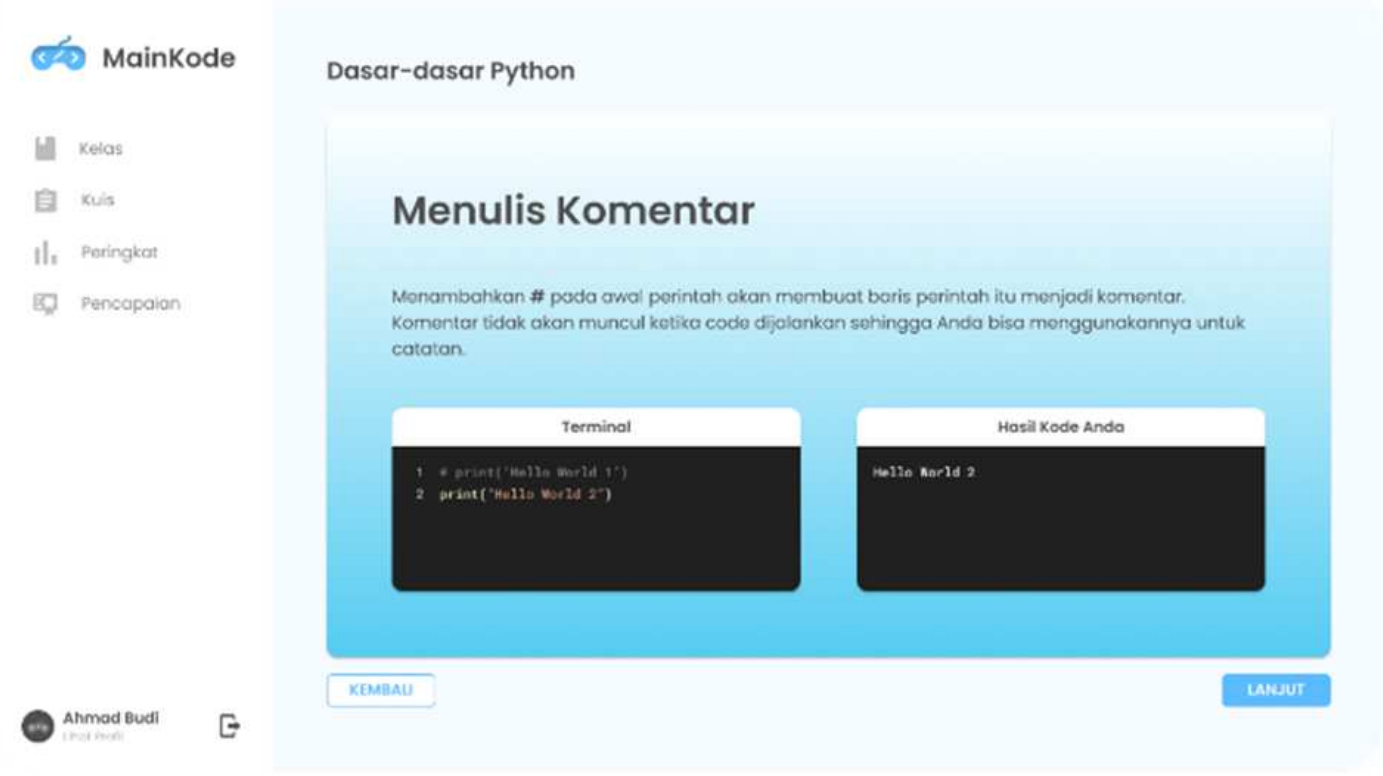
\includegraphics[width=\linewidth]{contents/chapter-2/images/Evan-a1.png}
	  \caption{\textit{Class topic page}}
	  \label{fig:sub1-a1}
	\end{subfigure}
	\begin{subfigure}[b]{0.4\textwidth}
	\centering
	  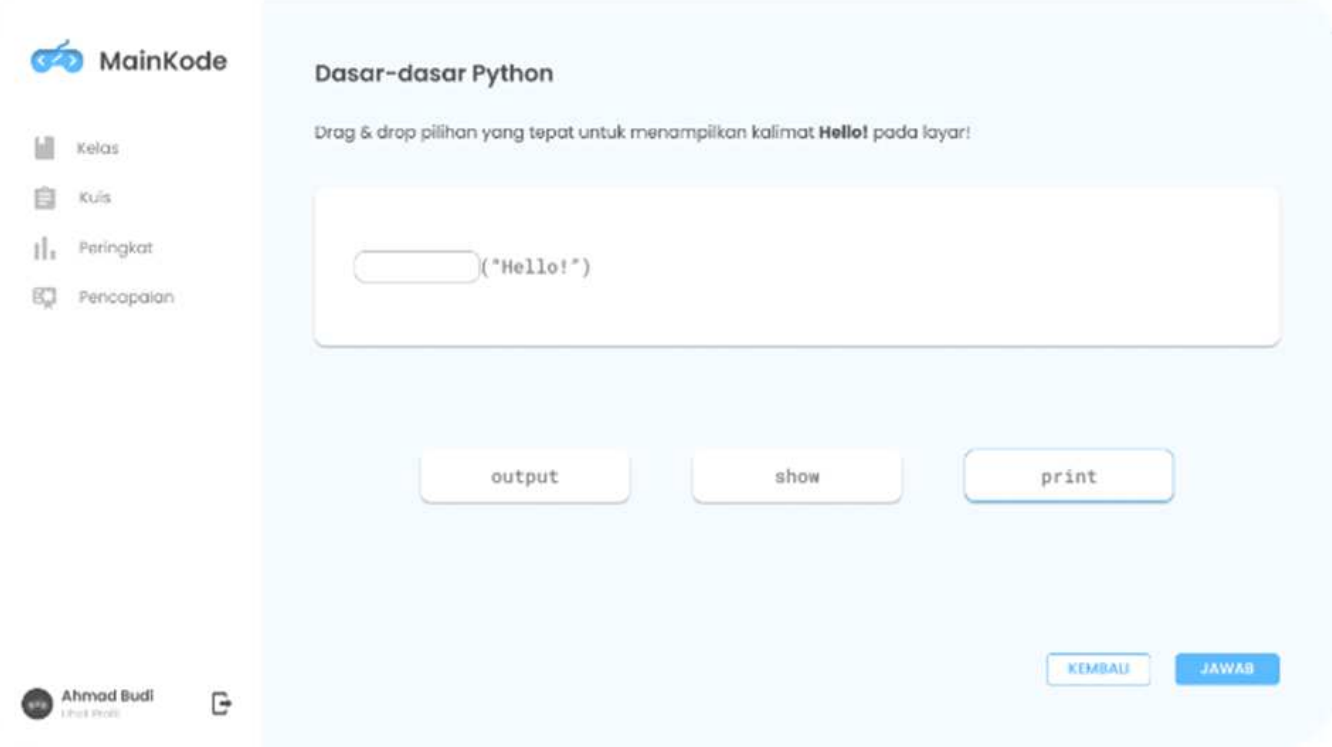
\includegraphics[width=\linewidth]{contents/chapter-2/images/Evan-a2.png}
	  \caption{\textit{Gamified exercise page}}
	  \label{fig:sub2-a2}
	\end{subfigure}
	\hfill
	\begin{subfigure}[b]{0.4\textwidth}
		\centering
		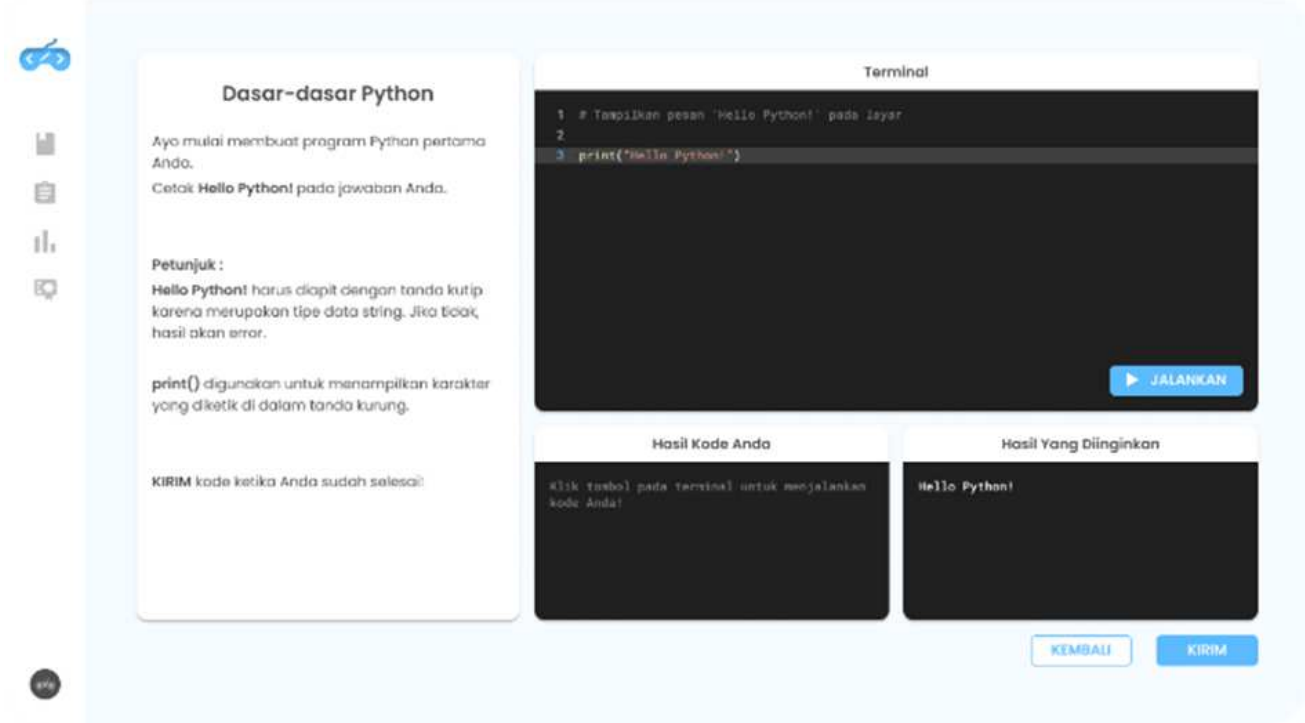
\includegraphics[width=\linewidth]{contents/chapter-2/images/Evan-a3.png}
		\caption{\textit{Terminal exercise page}}
		\label{fig:sub3-a3}
	\end{subfigure}  
	\begin{subfigure}[b]{0.4\textwidth}
		\centering
		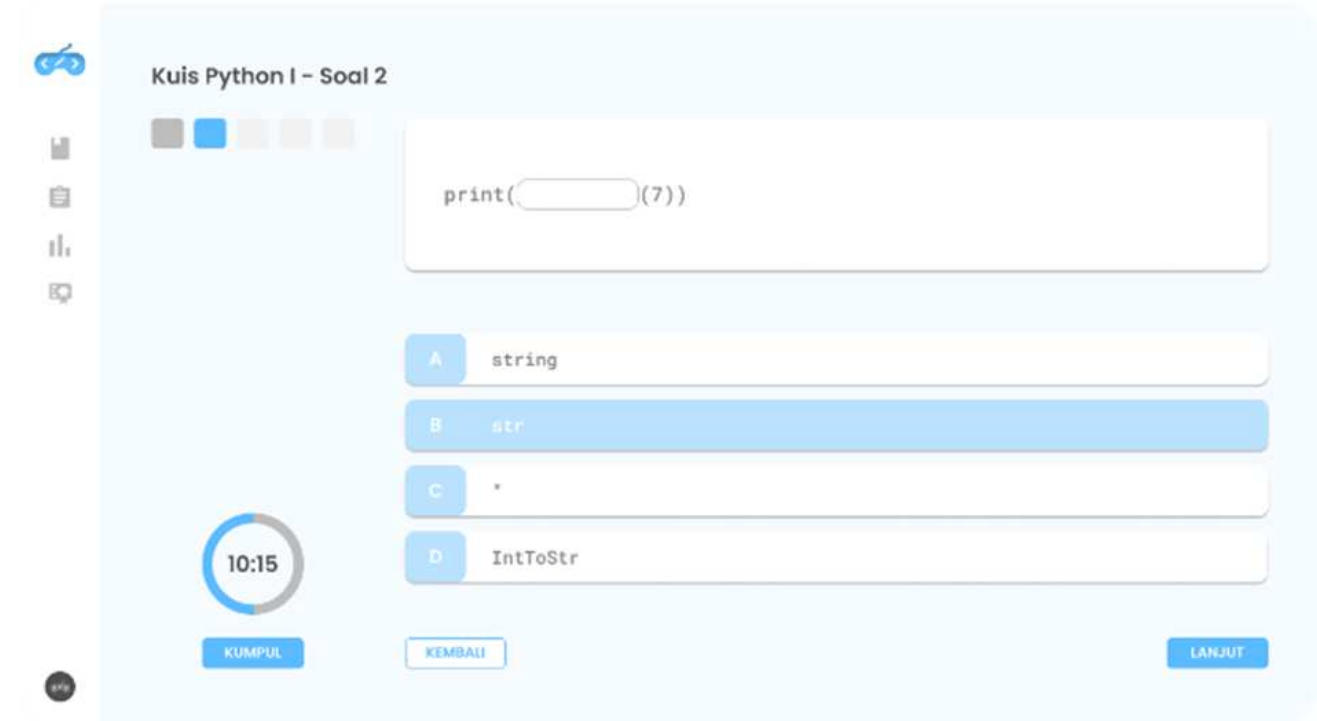
\includegraphics[width=\linewidth]{contents/chapter-2/images/Evan-a4.png}
		\caption{\textit{Quiz page}}
		\label{fig:sub4-a4}
	\end{subfigure} 
	\begin{subfigure}[b]{0.4\textwidth}
		\centering
		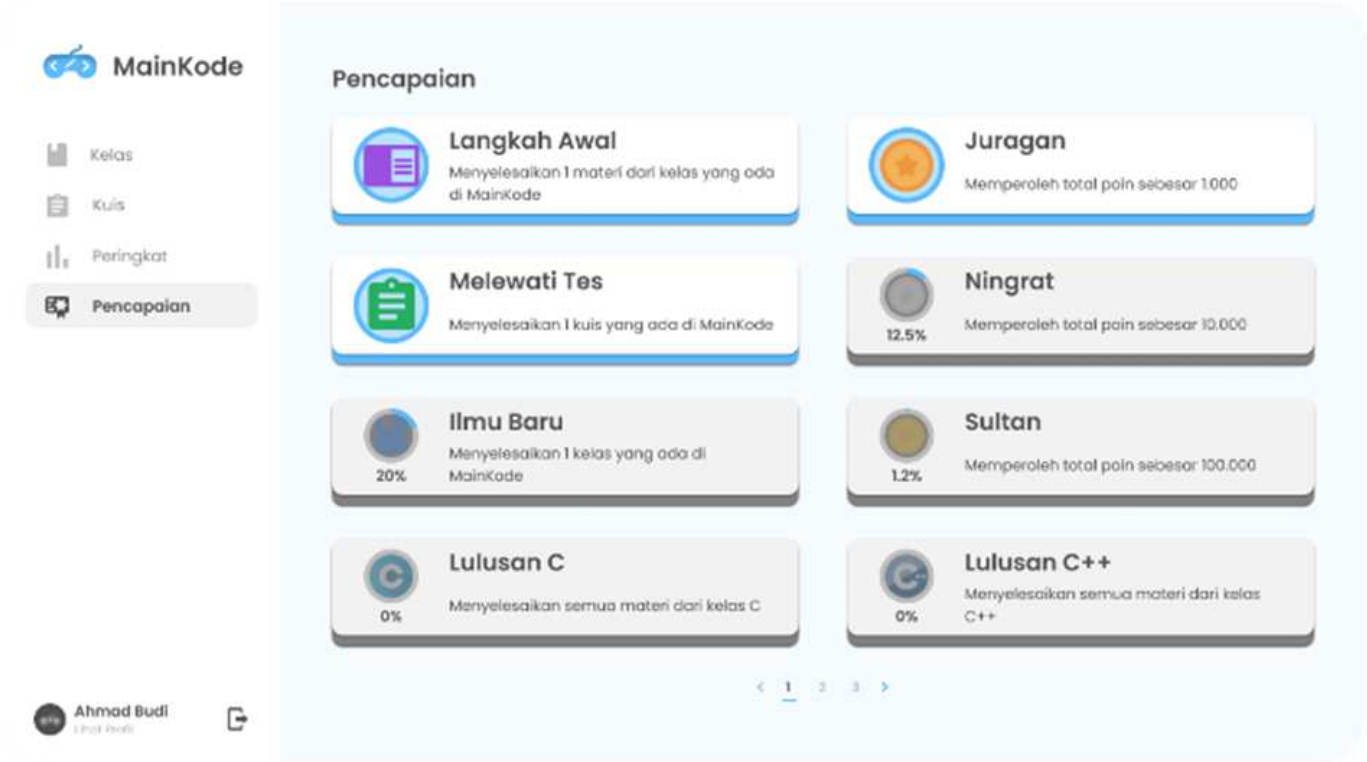
\includegraphics[width=\linewidth]{contents/chapter-2/images/Evan-a5.png}
		\caption{\textit{Achievement page}}
		\label{fig:sub5-a5}
	\end{subfigure} 
	\caption{\textit{High-fidelity prototype} aplikasi pembelajaran pemrograman}
	\label{fig:High-fidelity prototype Evan}
  \end{figure}
% ================================= Penelitian Design of Gamification for Anatomy Learning Media =================================
Ada juga penelitian yang dilakukan pada tahun 2021 oleh Bernadeta Ratna P. S. dan rekan-rekannya mengenai pengembangan desain gamifikasi ini.
Penelitian tersebut memaparkan mengenai pengembangan gamifikasi untuk sebuah media pembelajaran anatomi yang berjudul \textit{"Design of Gamification for Anatomy Learning Media"}.
Sama halnya dengan penelitian sebelumnya, penelitian ini memiliki tujuan untuk meningkatkan motivasi dan keterlibatan pengguna dalam memahami anatomi tubuh manusia.
Proses pengembangan desain gamifikasi pada penelitian ini menggunakan sebuah \textit{framework game design} yang dinamai \textit{"Elemental Tetrad"}.
\textit{Framework} memodelkan gamifikasi dalam 4 bentuk, yakni \textit{Mechanics},\textit{Aesthetics}, \textit{Story} atau \textit{Dynamics}, dan \textit{Technology}.
Masing masing elemen desain tersebut kemudian dikembangkan berdasarkan konteks pembelajaran yang akan dipelajari, dalam penelitian ini yaitu pembelajaran anatomi manusia.
\textit{Game Mechanics} dalam penelitiannya terdiri dari \textit{game mode}, \textit{parts}, \textit{points} dan\textit{reward}. 
Untuk elemen \textit{Aesthetics} terdiri dari \textit{ User Interface dan User Experience}, \textit{Art}, \textit{Unlocking Parts}, dan \textit{Challenges}.
Untuk \textit{Story}, akan mengikuti alur pembelajaran yang dibagi menjadi 3 bagian, yaitu materi, praktikum, dan kuis.
Untuk elemen terakhir yaitu teknologi yang digunakan dalam penelitian ini. Penelitian ini menggunakan \textit{Smartphone} dan 3D model dari kerangka manusia.
% \newpage
\begin{figure}[htbp]
	\centering
	\begin{subfigure}[b]{0.4\textwidth}
		\centering
	  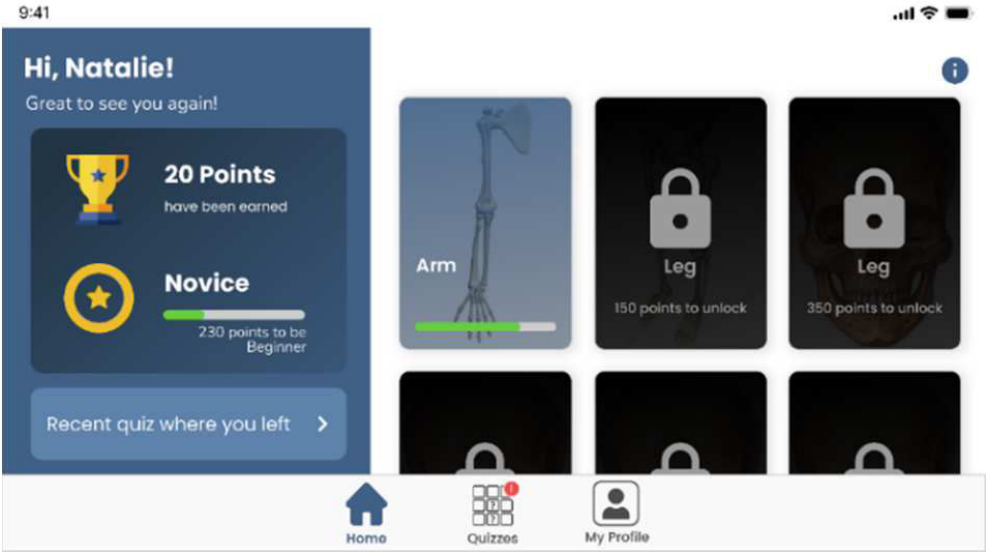
\includegraphics[width=\linewidth]{contents/chapter-2/images/Deta-a1.png}
	  \caption{\textit{Interface design home menu}}
	  \label{fig:sub-deta-a1}
	\end{subfigure}
	\begin{subfigure}[b]{0.4\textwidth}
	\centering
	  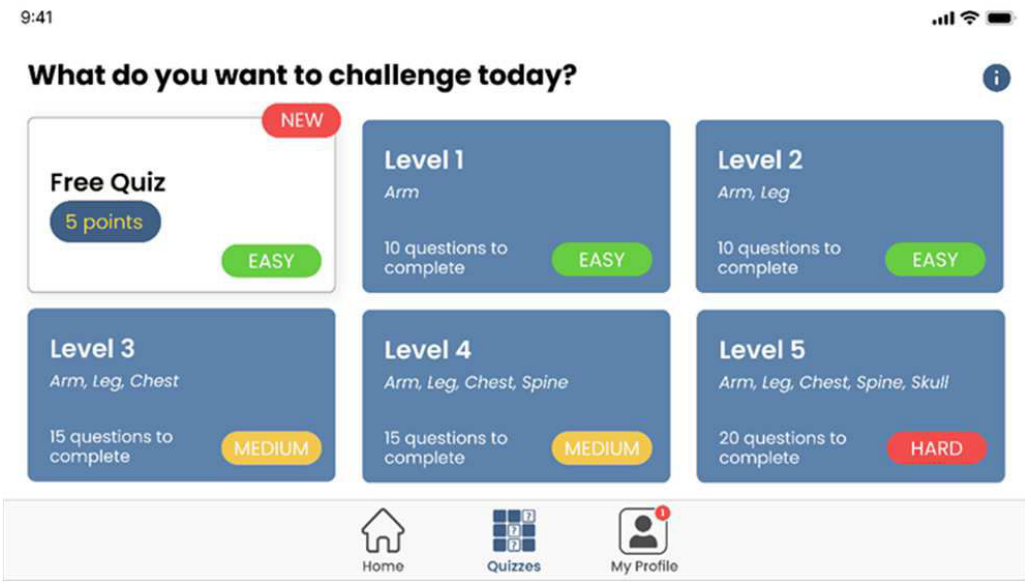
\includegraphics[width=\linewidth]{contents/chapter-2/images/Deta-a2.png}
	  \caption{\textit{Interface design quiz menu }}
	  \label{fig:sub-deta-a2}
	\end{subfigure}
	\hfill
	\begin{subfigure}[b]{0.4\textwidth}
		\centering
		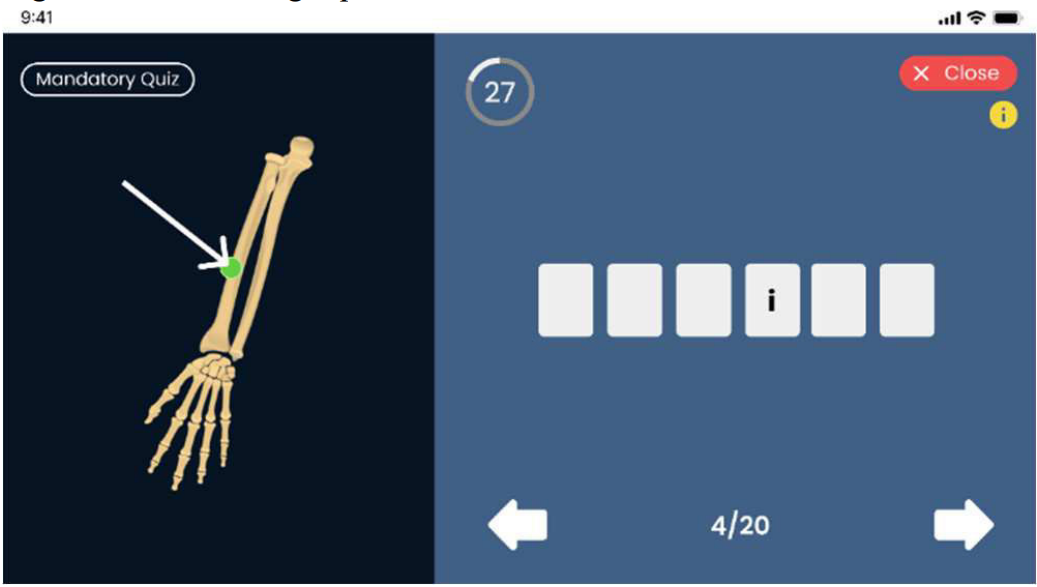
\includegraphics[width=\linewidth]{contents/chapter-2/images/Deta-a3.png}
		\caption{\textit{Interface design mandatory quiz}}
		\label{fig:sub-deta-a3}
	\end{subfigure}  
	\caption{Tampilam aplikasi pembelajaran anatomi}
	\label{fig:interface pembelajaran anatomi}
  \end{figure}
Hasil dari penelitianini berupa sebuah aplikasi \textit{Smartphone} yang dapat diinstall pada sistem operasi Android.
Tampilan aplikasi ini dilampirkan pada gamabar \ref*{fig:interface pembelajaran anatomi}.
Berbeda dengan penelitian sebelumnya, pada penelitian ini tidak dilakukan pengujian \textit{Usability} dan \textit{User Experience}.

Pengadaptasian gamifikasi pada sebuah media pembelajaran juga dijelasakan pada penelitian yang dilakukan oleh Andre Julian Irawan, Fenina Adline Twince Tobing, dan Eunike Endariahna Surbakti
dengan judul \textit{"Implementation of Gamification Octalysis Method at Design and Build a React Native Framework Learning Application"}.
Dalam penelitian ini, proses gamifikasi menggunakan kerangka kerja \textit{Octalysis} atau \textit{Octalysis Gamification Framework} untuk mengembangan sebuah aplikasi pembelajaran yang mempelajari \textit{React Native Framework}.
Kerangka kerja ini meruapakan sebuah kerangka kerja gamifikasi yang dikembangakan oleh Yu-Kai Chou, seorang ahli gamifikasi terkemuka[].
Metode \textit{Octalysis} memiliki delapan inti motivasi yang berfokus pada perilaku manusia, seperti \textit{meaning}, \textit{accomplishment}, \textit{empowerment}, \textit{ownership}, \textit{social influence}, \textit{scarcity}, \textit{unpredictability}, dan \textit{avoidance}.
Untuk mengukur keberhasilan dari penerapan gamifikasi yang dilakukan, penelitian ini mengerjakan beberapa pengujian untuk aplikasi yang dikembangkan.
Penelitian ini menggunakan \textit{Hedonic Motivation System Adoption Model (HMSAM)} untuk mengukur motivasi intrinsik dari sebuah sistem atau aplikasi.
Selain itu juga, dalam penelitian ini dialkukan pengukuran sikap, pendapat, dan persepsi seseorang tentang fenomena sosial dengan skala Likert atau \textit{Likert Scale}.
\newpage
\begin{figure}[htbp]
	\centering
	\begin{subfigure}[b]{0.4\textwidth}
		\centering
	  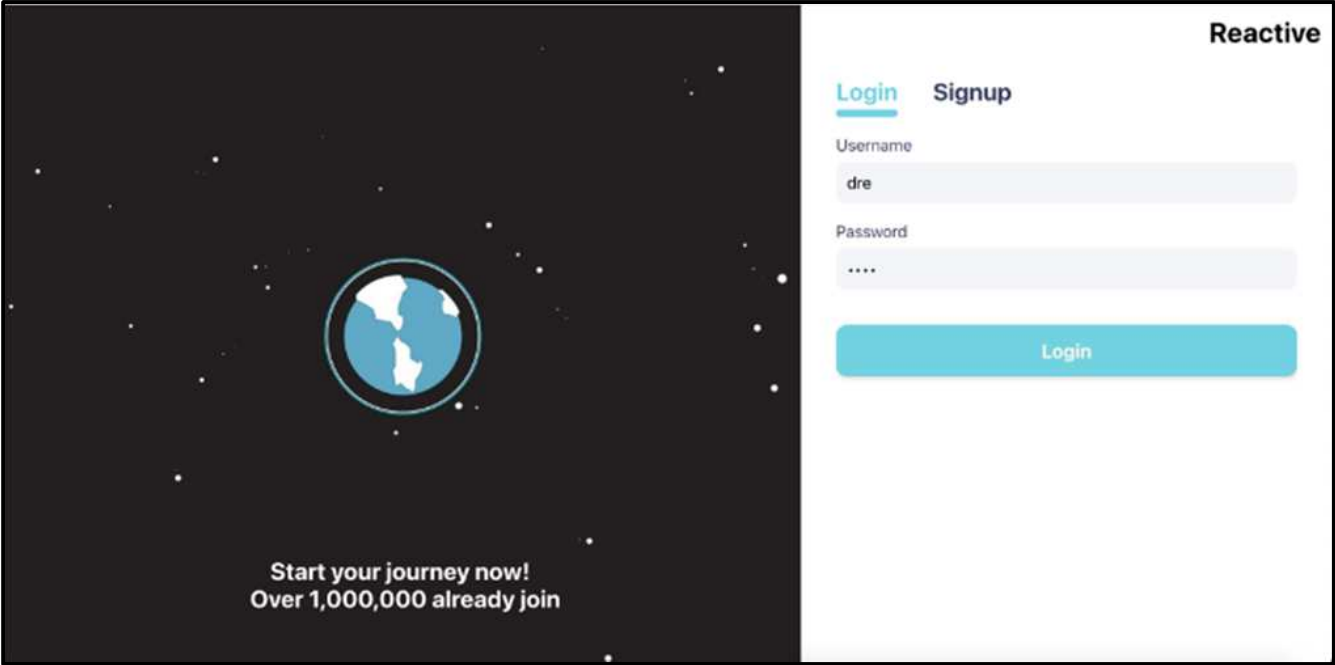
\includegraphics[width=\linewidth]{contents/chapter-2/images/Andre-a1.png}
	  \caption{\textit{Interface design home menu}}
	  \label{fig:sub-andre-a1}
	\end{subfigure}
	\begin{subfigure}[b]{0.4\textwidth}
	\centering
	  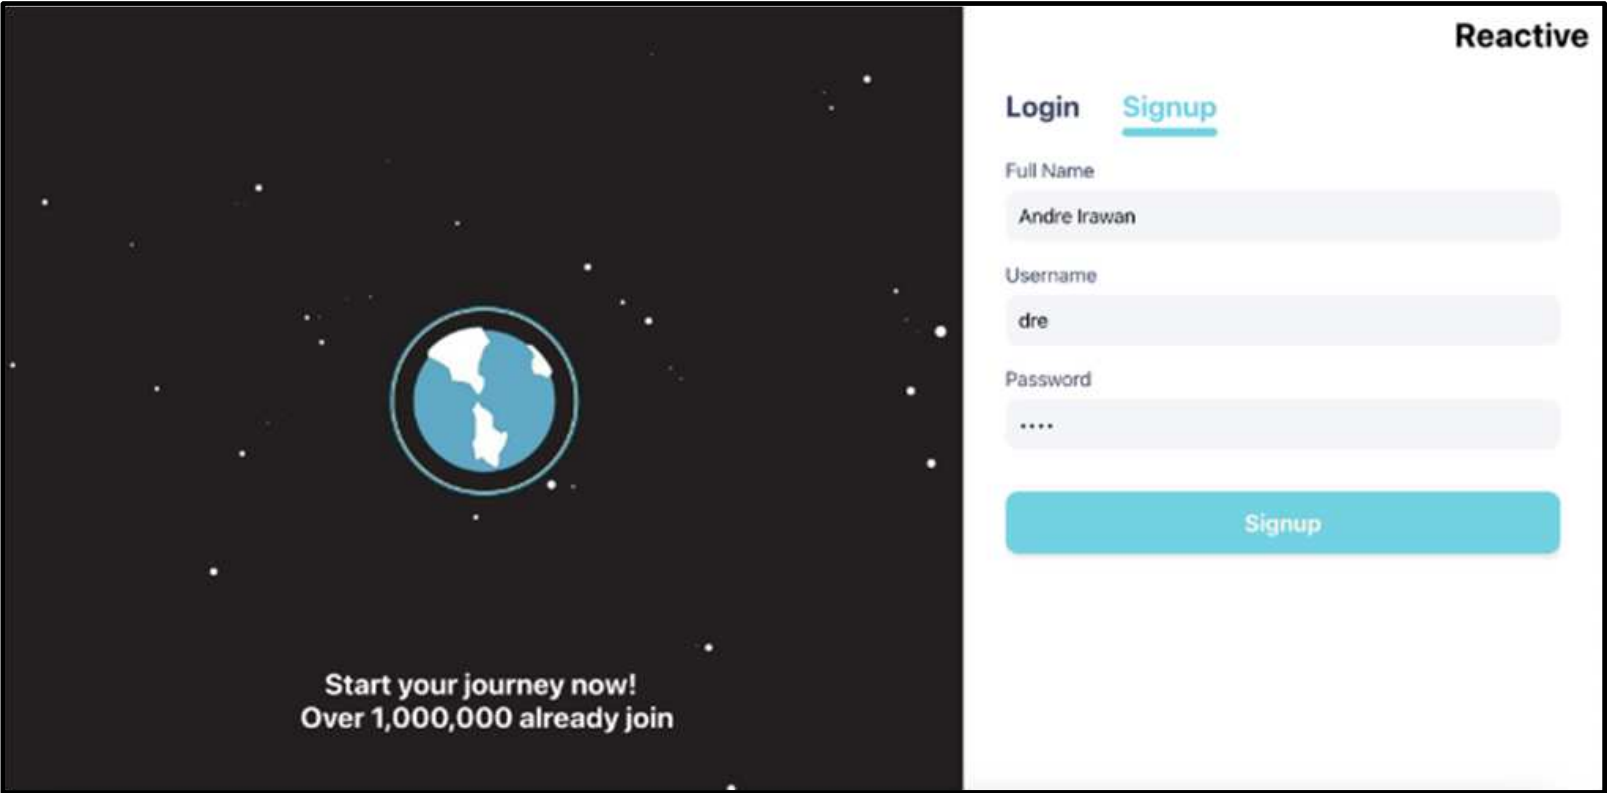
\includegraphics[width=\linewidth]{contents/chapter-2/images/Andre-a2.png}
	  \caption{\textit{Interface design quiz menu }}
	  \label{fig:sub-andre-a2}
	\end{subfigure}
	\hfill
	\begin{subfigure}[b]{0.4\textwidth}
		\centering
		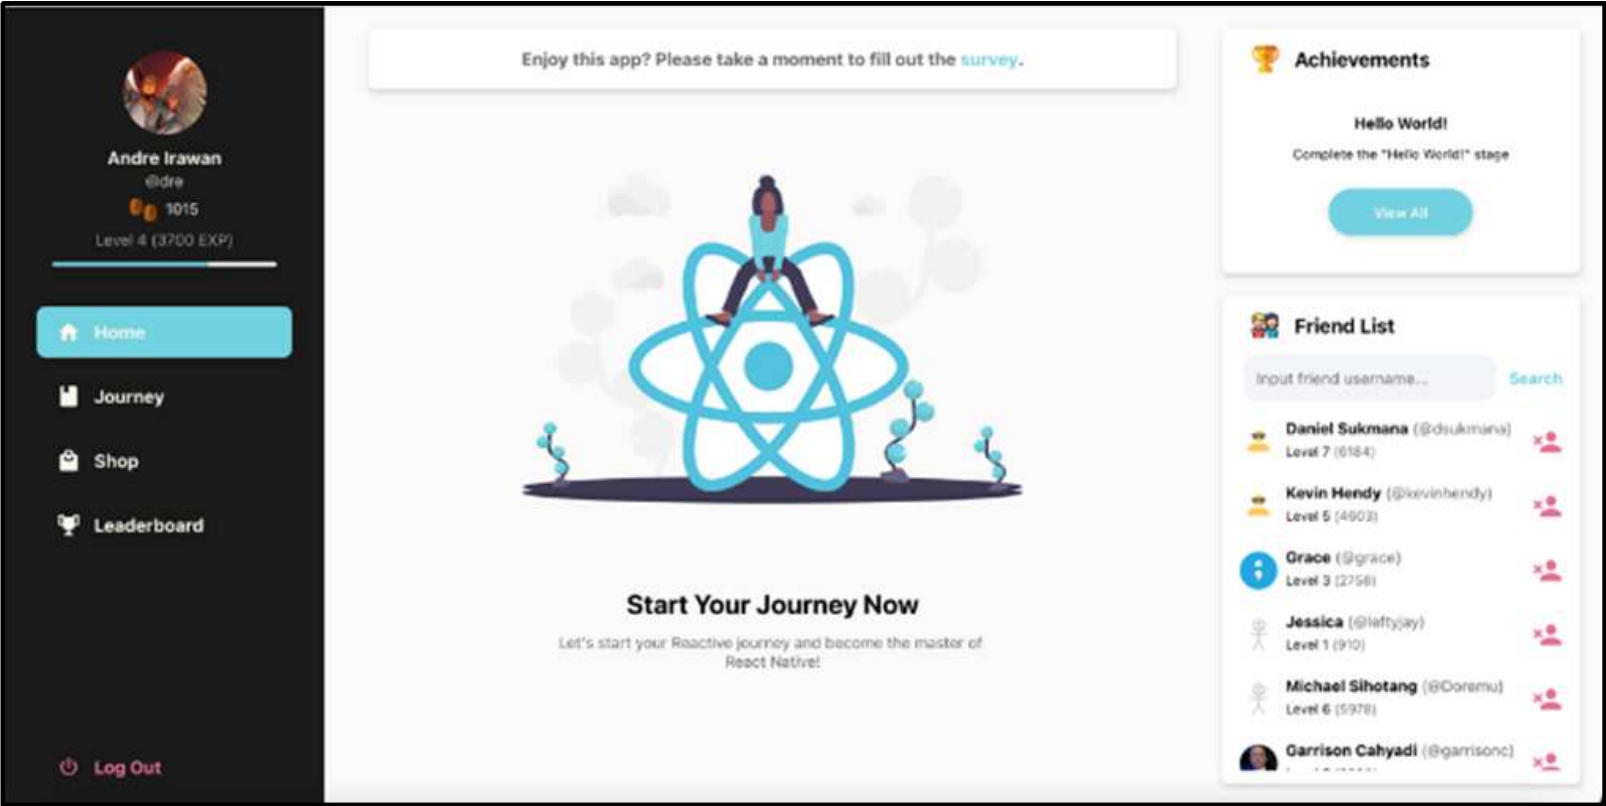
\includegraphics[width=\linewidth]{contents/chapter-2/images/Andre-a3.png}
		\caption{\textit{Interface design mandatory quiz}}
		\label{fig:sub-andre-a3}
	\end{subfigure}  
	\caption{Tampilam aplikasi pembelajaran \textit{React Native App}}
	\label{fig:interface pembelajaran React Native}
\end{figure}
\section{Analisis Perbandingan Metode}
Dari tinjauan pustaka yang dilakukan oleh penulis, penulis menemukan perbedaan metode desain dan pengembangan gamifikasi yang dugunakan pada setiap penelitian.
Perbedaan ini didasari dengan konteks pembelajaran yang akan dikembangkan, dan bagaimana aplikasi pembelajaran didesain dan dikembangkan.
Faktor lain perbedaan metode ini juga didasari oleh kebutuhan pengguna dan target device dimana aplikasi tersebut akan berjalan.
Penelitian yang dilakukan oleh Evan dan rekan-rekannya menggunakan metode \textit{Activity-centered Design} dimana metode ini dipilih karena aplikasi ini akan berfokus pada aktifitas utama pemrograman.
Berbeda halnya dengan penelitian yang dilakukan oleh Bernadeta dan rekan-rekan rekannya. Metode pengembangan aplikasi ini didasari dengan framework gamifikasi yang sudah ada sebelumnya yaitu \textit{Elemental Tetrad}.
Penelitian ini mendesain sebuah gamifikasi pembelajaran anatomi berdasarkan setiap elemen yang ada di \textit{Elemental Tetrad Framework}.
Penelitian yang dilakukan oleh Julian dan teman-temannya memiliki metode desain yang sama menggunakan sebuah kerangka kerja gamifikasi, 
bedanya  pada penelitiannya tersebut mereka menggunakan \textit{Octalysis} sebagai kerangka kerjanya. \textit{Framework} ini menggunakan 8 elemen yang fokus pada kebiasaan manusia.
Perbedaan antara kedua \textit{Framework} gamifikasi tersebut adalah dari tujuan kerangka kerjanya. Kerangka kerja \textit{Elemental Tetrad} berfokus pada pembentukan pengalaman Gamifikasi,
sedangkan \textit{Octalysis} berfokus pada pengaruh motivasi dan keterlibatan pengguna dalam gamifikasi. Perbadingan metode dapat dilihat dalam tabel \ref*{Tab: Tabel perbandingan metode}
% Metode tersebut dapat divisualisasikan dengan gambar \ref*{Fig:itterative-Design Cycle}
% \begin{figure}[H]
% 	\centering
% 	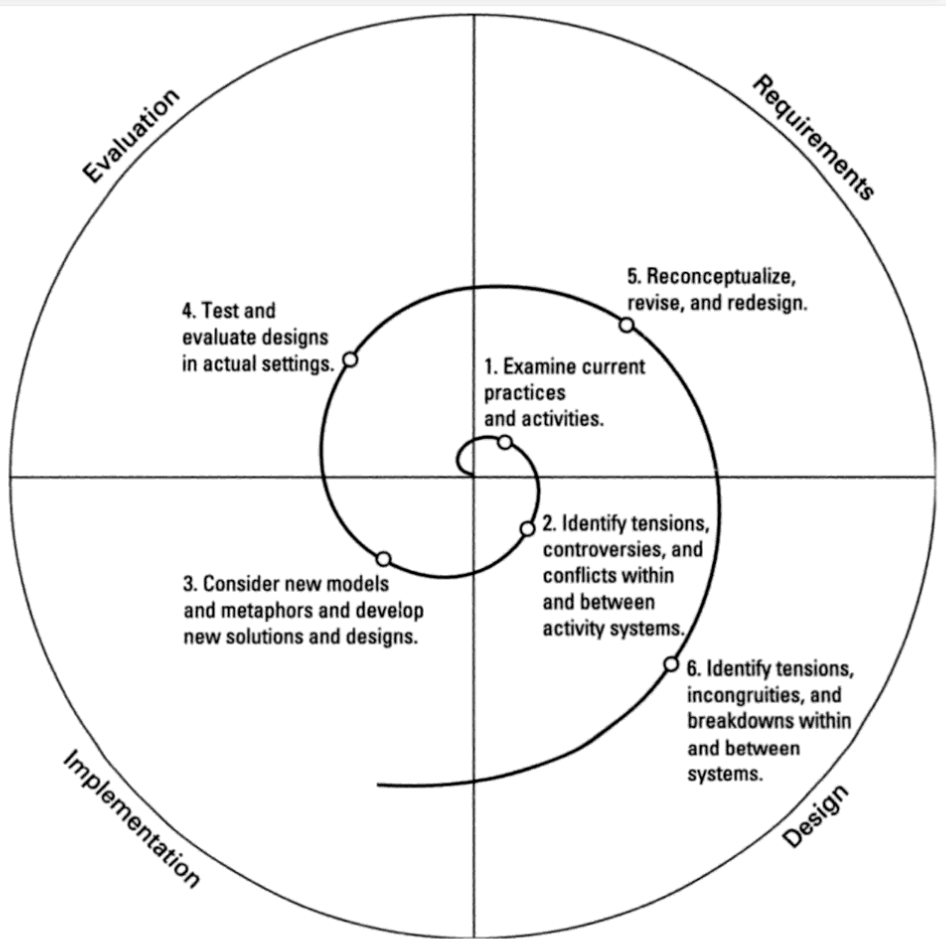
\includegraphics[width=6cm]{contents/chapter-2/images/Itterative-design.png}
% 	\caption[Caption]{An itterative-Design Cycle \cite{2004activity}}
% 	\label{Fig:itterative-Design Cycle}
% \end{figure}
\newpage
\begin{landscape}
	\begin{table}[htbp]
	\caption{Perbandingan Penelitian}
	\centering
	\begin{tabular}{|>{\centering\arraybackslash}m{0.5cm}|m{4cm}|m{3.5cm}|m{4.5cm}|m{4.5cm}|m{4cm}|m{4cm}|}
		\hline
		\centering \textbf{No} & \centering \textbf{Judul Penelitian} & \centering \textbf{Penulis} & \centering  \textbf{Pengembangan Desain Gamifikasi} &\centering\textbf{Fokus}&\multicolumn{1}{m{4cm}|}{\centering\textbf{Luaran}} \\
		\hline 
		1 & "\textit{Designing Gamification for Programming Learning Applications}"
		& 
		Evan Pradanika, Yani Widyani,  Yanti Rusmawati
		& \textit{Activity-centered Design} \& \textit{Type of Knowledge and Gamification Element Relation}& Merancang pengalaman pengguna yang optimal dengan memahami kebutuhan, konteks, dan tujuan aktivitas& \textit{High-fidelity Prototype} Aplikasi\\
		\hline
		2 &"\textit{Design of Gamification for Anatomy Learning Media}" 
		& 
		Adhistya Erna Permanasari, Bernadeta Ratna P S, Fikry Yanuar S, Mirza Putri Maharani, Sunu Wibirama, Junaedy Yunus
		& \textit{Elemental Tetrad Gamification Framework} & Membentuk pengalaman gamifikasi & Aplikasi Mobile\\
		\hline
		3 & 
		"\textit{Implementation of Gamification Octalysis Method at Design and Build a React Native Framework Learning Application}" 
		& 
		Andre Julian Irawan, Fenina Adline Twince Tobing, Eunike Endariahna Surbakti
		& \textit{Octalysis Gamification Framework}& Mempengaruhi Motivasi dan Keterlibatan pengguna & Aplikasi Web React Native\\
		\hline
	  \end{tabular}
	  \label{Tab: Tabel perbandingan metode}
	\end{table}
\end{landscape}

\newpage
\section{Dasar Teori}
\subsection{Media Pembelajaran}
Secara deskriptif, media pembelajaran merupakan sebuah medium yang memuat informasi atau pesan instruksional yang digunakan dalam proses pembelajaran\cite{hasan2021media}. 
Menurut \textit{Education Association} (NEA) mendefinisikan media pembelajaran sebagai benda yang dapat dimanipulasi, dilihat, didengar, dibaca atau dibicarakan 
beserta instrument yang dipergunakan dengan baik dalam kegiatan belajar mengajar, dapat mempengaruhi efektifitas program instruksional\cite{arsyad2011media}.
Media ini menjadi salah satu instrumen yang strategis dalam penentuan keberhasilan proses belajar mengajar. 
Keberadaan sebuah media pembelajaran dapat memberikan dinamika tersendiri terhadap peserta didik secara langsung.
Media pembelajaran sangat penting untuk membantu peserta didik memperoleh konsep baru, keterampilan dan kompetensi.
Ada banyak jenis media pembelajaran yang dapat diimplementasikan ke dalam sebuah pembelajaran, namun pemilihan media yang tepat akan berpengaruh pada hasil dari pembelajaran.
\subsubsection{Media Pembelajaran Elektronik}
Media Pembelajaran Elektronik atau yang lebih kita kenal sebagai \textit{E-Learning} merupakan sebuah media pembelajaran modern yang mengadopsi Teknologi Informasi untuk mempermudah penyampaian informasi.
Secara deskriptif, \textit{E-Learning} atau \textit{"Electronic learning} merupakan proses belajar dan mengajar degan menggunakan teknologi elektronik dan internet sebagai media pengirim dan penerima informasi.
Melalui media ini pengguna akan menggunakan perangkat elektronik seperti komputer, laptop, atau smartphone yang dapat mengakses internet untuk mengakses materi pembelajaran, berinteraksi dengan instruktur atau sesama peserta, dan menyelesaikan tugas-tugas atau ujian secara online.
\subsection{Gamifikasi}
Gamifikasi merupakan sebuah pendekatan yang mengadopsi elemen-elemen \textit{game} untuk menyelesaikan masalah non \textit{game} \cite{marisa2020gamifikasi}.
Konsep ini dapat berupa produk, cara berpikir, proses, pengalaman, cara desain, dan sistem dimana intinya ialah menggunakan elemen \textit{game} untuk menyelesaikan masalah non \textit{game}. 
Konsep gamifikasi tentu saja muncul dari karakteristik sebuah \textit{game entertainment} atau permainan yang secara harfiah dibuat untuk menghibur dan dapat menarik pengguna untuk mengoperasikannya.
Seiring perkembangan jaman, \textit{game entertainment} berkembag ke ranah yang lain seperti edukasi yang bertujuan untuk menarik pengguna untuk memotivasi pengguana.
Dengan demikian, konsep \textit{gamifikasi} ditemukan dan dapat diadopsi untuk menyelesaikan sebuah masalah. Visualisasi dari perkembangan ilmu seputar \textit{game} dapat di lihat pada gambar \ref*{Fig:Ilustrasi perkembangan ilmu game}.
\begin{figure}[H]
	\centering
	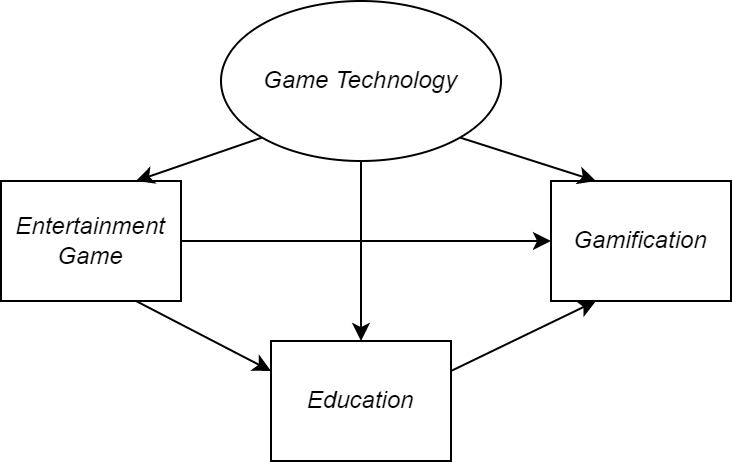
\includegraphics[width=7cm]{contents/chapter-2/images/perkembangan-game.png}
	\caption[Caption]{Ilustrasi perkembangan ilmu \textit{game} \cite{2004activity}}
	\label{Fig:Ilustrasi perkembangan ilmu game}
\end{figure}
\subsection{Game Thinking}
Game thinking merupakan sebuah pendekatan berpikir yang terinspsirasi oleh prinsip-prinsip desain dan mekanisme permainan dalam konteks non-game. 
Ini melibatkan penerapan elemen-elemen permainan, seperti tantangan, imbalan, persaingan, dan pencapaian, dalam lingkungan non-permainan seperti bisnis, pendidikan, atau pengembangan produk.
Pendekatan ini digunakan dalam proses Gamifikasi untuk menciptakan pengalaman yang lebih menyenangkan, menarik, dan efektif bagi pengguna atau peserta.
\begin{figure}[H]
	\centering
	\begin{subfigure}[b]{0.42\textwidth}
		\centering
	  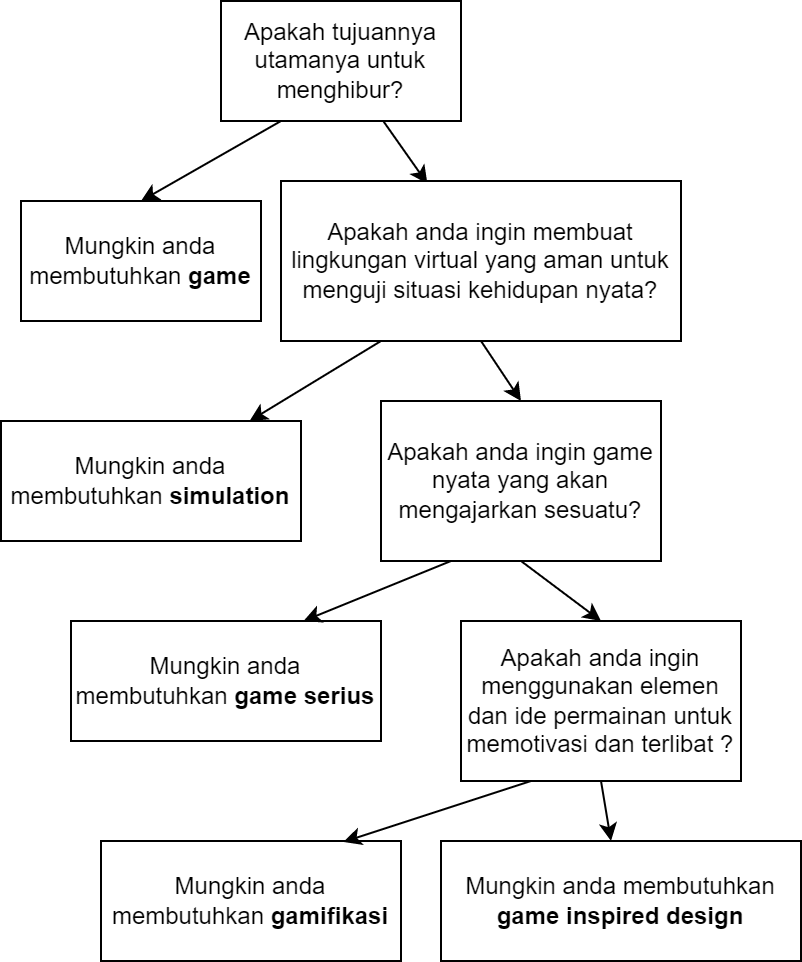
\includegraphics[width=\linewidth]{contents/chapter-2/images/Game-thinking-2.png}
	  \caption{\textit{game thinking}:Apa yang anda butuhkan}
	  \label{fig:sub-gamethink-1}
	\end{subfigure}
	\hfill
	\begin{subfigure}[b]{0.42\textwidth}
	\centering
	  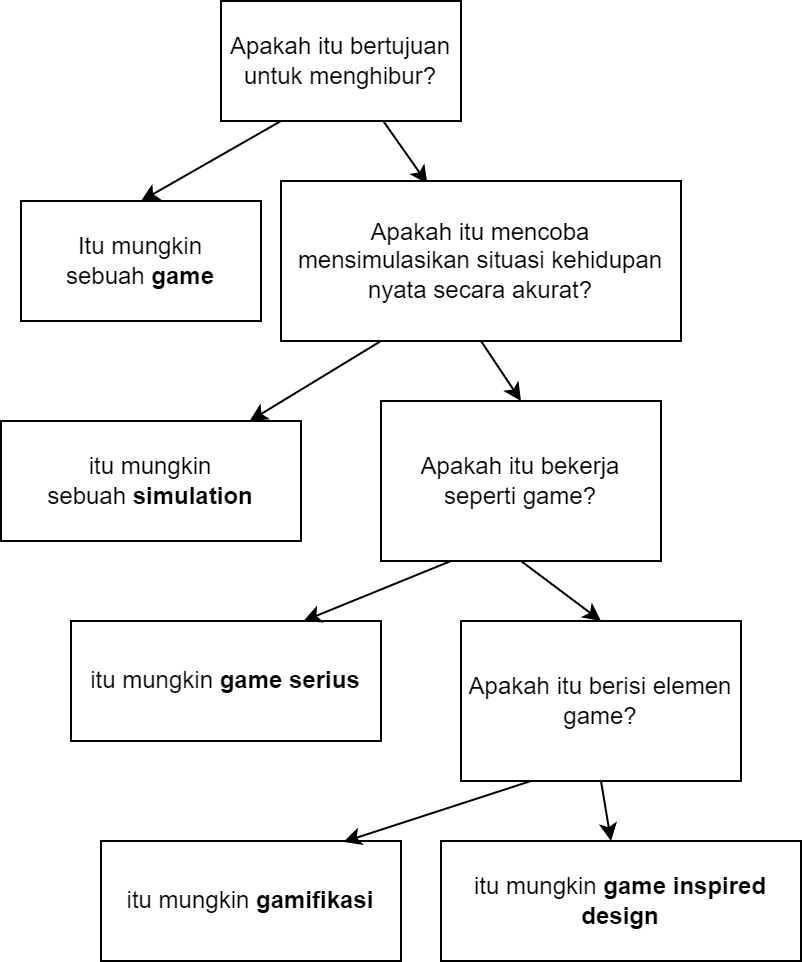
\includegraphics[width=\linewidth]{contents/chapter-2/images/Game-thinking-1.png}
	  \caption{\textit{game thinking}: Apa yang sudah anda dapatkan?}
	  \label{fig:sub-gamethink-2}
	\end{subfigure}
	\caption{\textit{Game Thinking}}
	\label{fig:Gamethink}
\end{figure}
Dengan konsep tersebut, kerangka kerja gamifikasi dikembangakan dengan tujuan memudahkan pengembangan gamifikasi secara terstruktur dan konsisten.
Kerangka kerja Gamifikasi yang ada saat ini adalah kerangka kerja Octalysis, MDA, Elemental Tetrad, MDE, dan SGD.
\subsubsection{\textit{The MDA Framework}}
MDA (Mechanics, Dynamics, Aesthetics) Framework adalah sebuah kerangka kerja yang digunakan dalam pengembangan permainan
(game development) untuk menganalisis dan memahami elemen-elemen inti yang membentuk pengalaman bermain game. 
Konsep ini pertama kali diperkenalkan oleh Robin Hunicke, Marc LeBlanc, dan Robert Zubek pada tahun 2004.
Dalam gamifikasi, pendekatan kereangka kerja ini secara formal digunakan dengan menganalisis desain game ke dalam 3 elemen,
Ketiga elemen tersebut diantaranya adalah \textit{Mechanics} yang menjelaskan aturan dan komponen permainan tertentu dalam hal tindakan, dan dapat disebut sebagai proses yang mendorong tindakan pengguna.
Kemudian \textit{Dynamics} sebagai elemen yang menguraikan cara implementasi aturan selama permainan game berdasarkan tindakan pemain yang diterjemahkan secara langsung ke dalam sistem, serta interaksi yang terjadi antara para pemain.
Lalu, ada juga \textit{Aesthetics} Menjelaskan respons emosional yang diharapkan yang timbul dari pengguna saat berinteraksi dengan sistem yang menggunakan gamifikasi.
\begin{figure}[H]
	\centering
	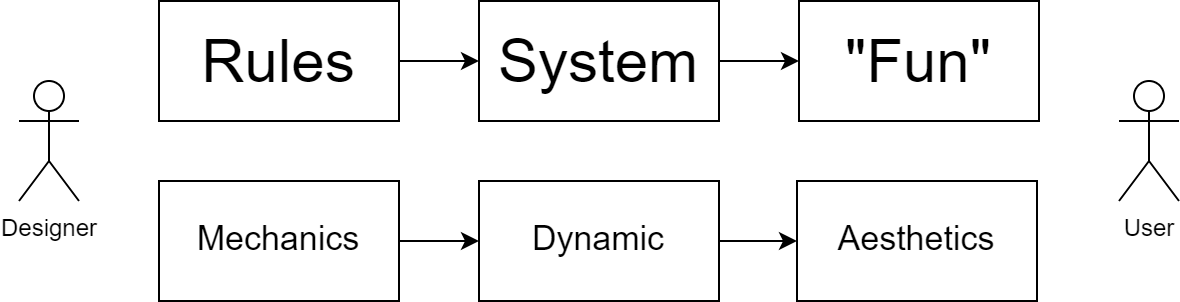
\includegraphics[height=4cm]{contents/chapter-2/images/MDA-framework.png}
	\caption[Caption]{Ilustrasi \textit{MDA Framework}}
	\label{Fig:Ilustrasi MDA}
\end{figure}
Gambar \ref*{Fig:Ilustrasi MDA} menunjukkan sebuah ilustrasi dari pengembanga gamifiakasi menggunakan kerangka kerja MDA.
Kerangka kerja MDA digambarkan sebagai hubungan satu arah dari desainer ke pengguna.
Kerangka kerja ini memungkinkan desainer membangun fungsi \textit{(Mechanics)} yang pada gilirannya menyediakan interaksi pengguna yang berbeda \textit{(Dynamics)}, yang membawa emosi dan pengalaman kepada pengguna \textit{(Aesthetics)}.
Biasanya, desainer lebih cenderung melihat permainan dari aspek mekanika \textit{(Mechanics)}, kemudian dinamika \textit{(Dynamics)}, dan terakhir estetika \textit{(Aesthetics)}, 
sedangkan pemain cenderung melihat ke arah yang berlawanan dimulai dari aspek estetika \textit{(Aesthetics)}, kemudian dinamika \textit{(Dynamics)}, dan terakhir mekanika \textit{(Dynamics)}.

Mekanika (Mechanics) berhubungan dengan elemen-elemen, kontrol, dan aturan yang diimplementasikan dalam permainan, seperti tindakan dasar, algoritma, mesin permainan, unsur-unsur permainan, dan sebagainya.
Mekanika melibatkan berbagai tindakan, algoritma, dan struktur data dalam mesin permainan yang secara keseluruhan mendukung dinamika dalam permainan.
Dinamika (Dynamics) menjelaskan bagaimana mekanika dalam permainan bekerja berdasarkan input dari pemain dan hubungannya dengan mekanika lainnya.
Dinamika (Dynamics) memiliki potensi untuk menciptakan estetika (Aesthetics) bagi siapa pun yang memainkan game. Estetika ini dapat berupa kepuasan, kekecewaan, kebimbangan, keragu-raguan, dan berbagai perasaan lainnya yang timbul selama permainan.
\subsection{\textit{Activity-centered Design}}
\textit{Activity-centered Design} atau (ACD) merupakan metode desain sebuah sistem yang pendekatannya berfokus pada perilaku yang berkaitan dengan tugas tertentu.
Pendekatan ini cocok untuk mendesain sebuah sistem yang memerlukan tindakan kompleks dengan pengguna yang beragam.
Untuk metode pengembangan desainnya sendiri, \textit{Activity-centered Design} menggunakan \textit{Iterative Design Cycle} yang terlampir pada gambar \ref*{Fig:itterative-Design Cycle}
\begin{figure}[H]
	\centering
	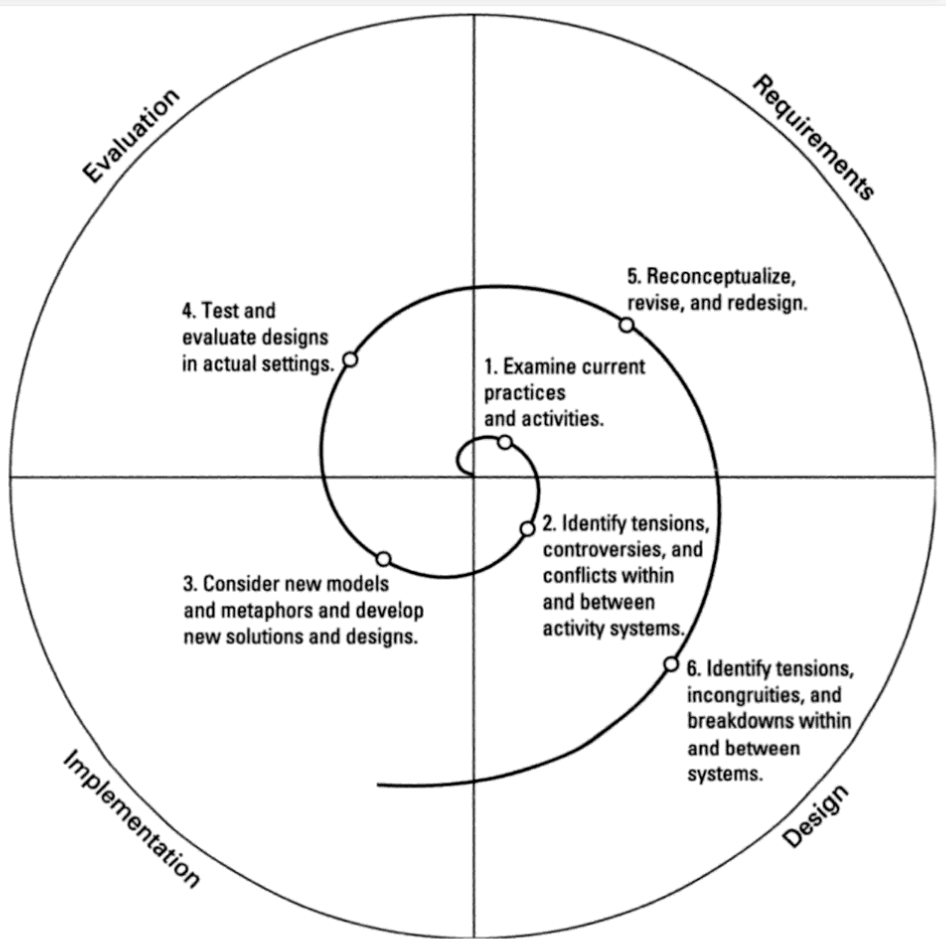
\includegraphics[height=8cm]{contents/chapter-2/images/Itterative-design.png}
	\caption[Caption]{An itterative-Design Cycle \cite{2004activity}}
	\label{Fig:itterative-Design Cycle}
\end{figure}
Tahap pertama pada metode ini ialah tahap \textit{Requirements}. Pada tahap ini, dilakukan identifikasi kebutuhan dan aktivitas. 
Kemudian pada tahap Desain \textit{Design}, dilakukan identifikasi dan penyelesaian konflik yang mungkin timbul antara aktivitas dalam sistem.
Selanjutnya pada tahap \textit{Implementasi}, solusi dan desain dikembangkan dan dievaluasi pada tahap \textit{Evaluation}
Akhirnya, siklus tersebut diulang hingga kebutuhan sistem tercapai.
\subsection{\textit{Feature-Driven Development}}
\textit{Feature-Driven Development} (FDD) adalah metode pengembangan perangkat lunak yang mengadopsi pendekatan iteratif dan merupakan salah satu pendekatan dalam kerangka metodologi \textit{Agile}.
Proses pengembangan perangkat lunak ini terdiri dari 5 aktivitas utama, yaitu \textit{Develop Overall Model}, \textit{Plan by Features}, \textit{Design by Features}, dan \textit{Build by Features}.
5 aktivitas tersebut divisualisasikan oleh gambar \ref*{Fig:FDD-langkah}
\begin{figure}[H]
	\centering
	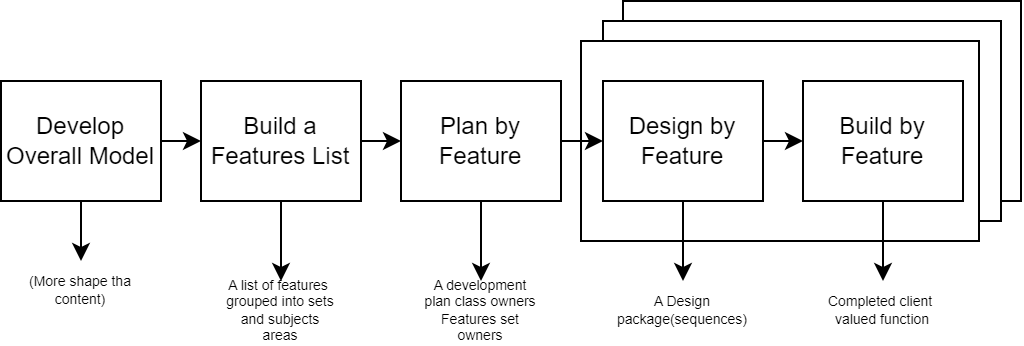
\includegraphics[width=\textwidth]{contents/chapter-2/images/FDD.png}
	\caption[Caption]{Aktivitas utama \textit{Feature-driven Development}\cite{palmer2001practical}}
	\label{Fig:FDD-langkah}
\end{figure}
Aktivitas yang pertama ialah \textit{Develop Overall Model}, proses ini merupakan proses identifikasi dan memahami dasar permasalahan yang akan ditangani oleh perangkat lunak yang akan dikembangakan.
Hasilnya berupa \textit{high-level object model} yang sepanjang proses pengembangan akan terus disempurnakan. Dilanjutkan dengan proses \textit{Build a Features List} dengan membuat daftar fitur yang akan dikembangkan dan mengelompokkannya ke dalam kelompok atau set terkait.
Kemudian, proses \textit{Plan by Feature} merupakan aktivitas yang menentukan pemilik dari suatu \textit{Class} atau kelompok fitur.
Setelah itu, untuk proses \textit{Design by Feature} dan \textit{Build by Feature} merupakan proses \textit{modeling} yang lebih detail hingga mendapatkan hasil yang sesuai dengan kebutuhan.
Proses \textit{modeling} tersebut termasuk pengembangan kode, dan \textit{testing system}.
\subsection{\textit{Black Box Testing}}
Black Box
\subsection{\textit{System Usability Testing}(SUS)}
system Usability
\subsection{\textit{User Experience Questionnaire}(UEQ)}
User Experience

% Di dalam tinjauan pustaka hasil akhirnya adalah analisis secara kualitatif atau pun secara kuantitatif kelebihan dan kekurangan metode jika dikaitkan dengan masalah, batasan-batasan masalah dan solusi yang dinginkan.
% Analisis kuantitatif tidak wajib teapi mempunyai nilai tambah di dalam tugas akhir saudara. Bagian ini menjelaskan kenapa metode tersebut dipilih dan uraikan dengan lebih jelas metode pelaksanaan tugas akhir yang ingin Anda lakukan. 
% \section{Pertanyaan Tugas Akhir (Jika Perlu)}

% Pertanyaan tugas akhir bersifat opsional dan dapat ditambahkan untuk menekankan hal-hal yang hendak diketahui dari tugas akhir berdasar pada tujuan tugas akhir. Pertanyaan tugas akhir dikenal dengan RQ (\textit{Research Question}) dan harus memiliki keterkaitan dengan RO (\textit{Research Objective}). Satu RO dapat memiliki satu atau lebih dari satu RQ. 

